% !TEX root = deckblatt3b.tex

\section{Integrierer}
\subsection{Aufgabenstellung}
Es soll ein Integrier aufgebaut werden und dessen Funktion gepr\"uft werden. Anschlie\ss{}end soll die Funtkion des Integrierers erl\"autert werden.
\subsection{Schaltung}
\begin{figure}[H]
  \begin{center}
    %\tikzset{component/.style={draw,thick,circle,fill=white,minimum size =0.75cm,inner sep=0pt}}
      \begin{circuitikz}
      \draw
      (-2,2) node[ground] (ground) {}
      (3,4) node[op amp] (opamp) {}
      (3,4.5) to[short] (3,5) node[vcc] {$V_{CC}$}
      (3,3.5) to[short] (3,3) node[vss] {$V_{SS}$}
      (opamp.-) to[R={$R$}{$=2,2k$}] (-2,4.5)
      (opamp.+) to[short] (1.5,3.5) to[short] (1.5,2) node[ground] (ground) {}

      (1.5,4.5) to[short] (1.5,6.5) to[C={$C$}{$=1\mu$}] (4.5,6.5) to[short] (4.5,4)
      (1.5,6.5) to[short] (1.5,8) to[R=$220k$] (4.5,8) to[short] (4.5,6.5)
      (opamp.out) to[short] (6,4)
      (6,2) node[ground] (ground) {}
      ;
      \draw (-2,4.2) to[short] (-2,2.7) node[vee] {};
      \draw (-1.5,3) node[] {$U_e$};
      \draw (6,3.7) to[short] (6,2.7) node[vee] {};
      \draw (6.5,3) node[] {$U_a$};
      \end{circuitikz}
    \caption{nicht inververtierender OPV}
  \end{center}
\end{figure}
\noindent
F\"ur die Schaltung des Integrierers wird die Grundschatung des invertierenden Verst\"arkers verwendet, es wird lediglich der R\"uckkopplungs Widerstand durch einen Kondensator ersetzt. Der Widerstand parallel zum Kondensator wird um vieles gr\"o\ss{}er gew\"ahlt als der Widerstand am Eingang (in der Regel $10*R_1$). Dieser beeinflusst die Schaltungseigenschaften nicht, er dient der Entladung des Kondensator vor dem Eingangszeipunkt um die Anfangsbedingung ($U_a=0V$) des Integrators zu bewerkstelligen.
\newpage
\subsection{Messung im Zeitbereich}
F\"ur die Messung im Zeitbereich wurde am Eingang ein Rechtecksignal mit $f=5Hz$ und einer Amplitude von $0.1Vpp$ angelegt.

\begin{figure}[H]
 \begin{center}
  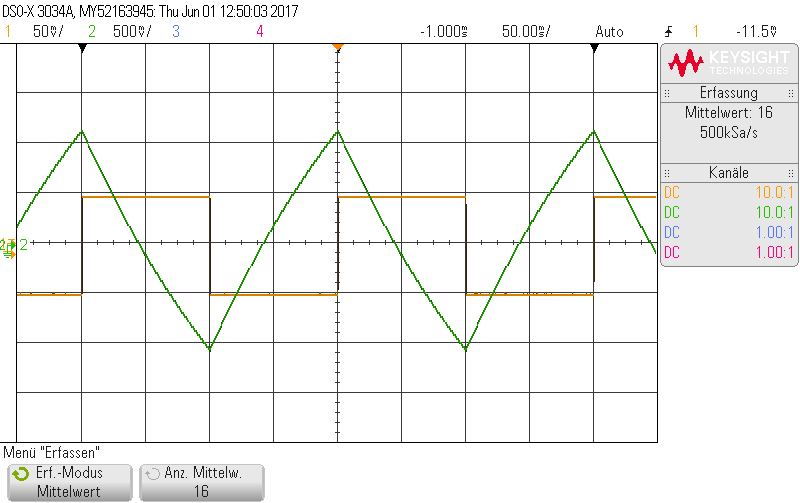
\includegraphics[height=6cm,width=12cm]{OsziBilder/invInte_bigScal.png}
 \end{center}
 \caption{Rechteckspannung $0,1V_{pp}$, $5Hz$ ($U_e$ orange, $U_a$ grün)}
\end{figure}
Jede Halbwelle des Eingangssinales entspricht einen Sprung und ein Sprung integriert ergibt eine Gerade. Da es sich um einen invertierenden Integrierer handelt l\"auft die Gerade immer entegen des Sprunges. In der Abbildung ist genau dieses Verhatlen sehr gut zu erkennen, springt die Eingangspannung ins Negative, entspricht die Ausgnagsspannung einer Gerade mit positiver Steigung, springt die Eingangsspannung ins Positive ist die Ausgangsspannung eine Gerade mit negativer Steigung.
\newpage
\subsection{Erl\"auterung der Schaltung}
\begin{figure}[H]
  \centering
  \begin{tabular}{ccc}
    & & Ohm'sches Gesetz an $C$ \\
    & & $I=C*\frac{du}{dt}$ \\ \\
    Ohm'sches Gesetz an $R$& & $du = \frac{I*dt}{C}$ \\ \\
    $I=\frac{U_e}{R}$ & & $U_a=\frac{1}{C}\int I dt$ \\
    & Zusammenf\"uhrung der Formeln & \\
    & $U_a = -\frac{1}{C} \int \frac{U_e}{R} dt$ & \\ \\
    & $U_a = -\frac{1}{RC} \int U_e dt$ & \\
  \end{tabular}
  \caption{Formeln zur Berechnung des Integrierers}
\end{figure}
\noindent
Da auf Grund des hohen Eingangswiderstandes kein Strom in den OPV flie\ss{}t, flie\ss{}t durch den Widerstand und den Kondensator quasi der gleiche Strom. Dieser Strom l\"asst sich sowohl am Widerstand als auch am Kondensator durch das Ohm'sche Gesetz berechnen. Formt man nun das Ohm'sche Gesetz von $C$ nach $du$ um, so erh\"alt man eine Differntialgleichung 1. Ordnung. Diese l\"asst sich durch Integrieren l\"osen und es ergibt sich eine Formel zur Berechnung von $U_a$. Setzt man nun die Berechnung f\"ur $I$ am Widerstand in die Umgeformte Formel von $C$ ein erh\"alt man die Formel zur Berechnung der Ausgangsspannung. \\ \\
$U_a = -\frac{1}{RC} \int U_e dt$ \\  \\
Diese Formel besagt, dass die Ausgangsspannung das Integral der Eingangsspannunt mit dem Proportionalit\"atsfaktor $\frac{1}{RC}$ ist. \\ \\
Mithilfe des Integrieres k\"onnen, wie der Name schon sagt, Integrale gel\"ost werden. Diese Schaltung wird in der Regelungstechnik f\"ur Integralrelger verwendet (PI-, PID-Regler).

\newpage
